\chapter{Fenomeni d'urto}
Si consideri l'urto tra due punti materiali. Durante il fenomeno si possono sviluppare forze molto intense che modificano la quantità di moto di ciascun punto. Queste forze, che agiscono per un breve intervallo di tempo rispetto a quello di osservazione del fenomeno, prendono il nome di forze impulsive. L'azione della forza si esplica nell'intervallo $\tau=t_1-t_1$. Le forze che si manifestano durante il processo d'urto sono forze interne. Quindi, in assenza di forze esterne, durante l'urto si verifica la conservazione della quantità di moto totale.

Indicando con $\vv_{1,i}$ e $\vv_{2,i}$ le velocità nell'istante precedente all'urto dei due punti materiali, di masse $m_1$ e $m_2$, e con $\vv_{1,f}$ e $\vv_{2,f}$ le corrispondenti velocità successive all'urto, la conservazione di $\vp$ si esprime come
\begin{equation}
    \vp_i=m_1\vv_{1,i}+m_2\vv_{2,i}=m_1\vv_{1,f}+m_2\vv_{2,f}=\vp_f.
\end{equation}
La quantità di moto del centro di massa rimane invariata
\begin{equation}
\label{eq: conservazione impulso CM urto 2 punti}
    \vp=(m_1+m_2)\vcm=\vp_i=\vp_f=costante.
\end{equation}
Quindi, il moto del centro di massa non viene modificato dall'urto dei due punti. Invece, variano le quantità di moto di ciascun punto materiale per effetto dell'impulso della forza di interazione secondo
\begin{align}
    \Delta\vp_1&=m_1\vv_{1,f}-m_1\vv_{1,i}=\int_{t_1}^{t_2}\vF_{2,1}\,dt=\vJ_{2,1} \\
    \Delta\vp_2&=m_1\vv_{2,f}-m_1\vv_{2,i}=\int_{t_1}^{t_2}\vF_{1,2}\,dt=\vJ_{1,2}.
\end{align}
Naturalmente
\begin{equation}
    \vF_{1,2}=-\vF_{2,1}\Rightarrow\vJ_{1,2}=-\vJ_{2,1},\quad\Delta\vp_1=-\Delta\vp_2,
\end{equation}
ossia le variazioni di quantità di moto sono uguali e opposte. 

Si può conservare la quantità di moto totale se sono presenti forze esterne? La risposta è sì se la durata dell'urto $\tau$ è sufficientemente breve e se le forze esterne non sono impulsive. Infatti, la variazione di $\Delta\vp$ in presenza di forze esterne è
\begin{equation}
\begin{split}
    \Delta\vp&=\Delta\vp_1+\Delta\vp_2=\int_{t_1}^{t_2}(\vF_{2,1}+\vF^{ext}_1)\,dt+\int_{t_1}^{t_2}(\vF_{1,2}+\vF^{ext}_2)\,dt \\
    &=\vJ_{2,1}+\vJ_{1,2}+\int_{t_1}^{t_2}\vF^{ext}\,dt=\vmedio{\vF^{ext}}\tau,
\end{split}
\end{equation}
dove se $\tau\to0$, allora anche $\Delta\vp\to0$. Se invece $\vF^{ext}$ fosse impulsiva in $\tau$, il valore medio $\vmedio{\vF^{ext}}$ potrebbe assumere valori molto alti, rendendo $\Delta\vp$ non trascurabile. La forza esterna non modifica i singoli impulsi durante l'urto quindi rimane vera l'uguaglianza $\vJ_{1,2}=-\vJ_{2,1}$ e quindi la conservazione della quantità di moto totale. Riassumendo, un urto è definito dalle seguenti proprietà:
\begin{enumerate}
    \item consiste in uno scambio di quantità di moto tra due punti materiali sotto forma di impulsi dovuti alle forze interne tra di essi;
    \item la quantità di moto totale si conserva.
\end{enumerate}
Queste caratteristiche prescindono dal meccanismo con il quale avviene l'urto e quindi dall'effettivo contatto tra i due punti. 

Tuttavia, a priori non è possibile sapere se le forze interne sono conservative e pertanto non si può applicare il principio di conservazione dell'energia meccanica. Dato che la posizione dei due punti durante l'urto non varia, le rispettive energie potenziali non variano e quindi $\Delta E=\Delta K$. Applicando il secondo teorema di K\"onig si ha
\begin{equation}
    K=\frac{1}{2}(m_1+m_2)\vcm^{\ 2}+K'.
\end{equation}
Il primo termine è l'energia cinetica del centro di massa, la quale non varia se si conserva la quantità di moto totale, mentre il secondo termine è l'energia cinetica rispetto al centro di massa, la quale può variare o meno a seconda che le forze interne siano non conservative o conservative, definita da
\begin{equation}
    K'=\frac{1}{2}m_1(v_1')^2+\frac{1}{2}m_2(v_2')^2.
\end{equation}

\section{Sistemi di laboratorio e centro di massa}
Per studiare gli urti i sistemi di riferimento più comuni sono quello del laboratorio e quello del centro di massa. Il legame tra le velocità in qualsiasi istante tra questi due è
\begin{equation}
\label{eq: legame velocità SdRL e SdRCM}
    \vv_1=\vvi_1+\vcm,\quad\vv_2=\vvi_2+\vcm.
\end{equation}
Nel sistema del centro di massa la quantità di moto totale è nulla, infatti, da $\vp=m_1\vv_1+m_2\vv_2$, usando \eqref{eq: conservazione impulso CM urto 2 punti} e \eqref{eq: legame velocità SdRL e SdRCM}, si ha
\begin{equation}
    \begin{split}
            \vp&=m_1\vvi_1+m_2\vvi_2+(m_1+m_2)\vcm\Rightarrow m_1\vvi_1+m_2\vvi_2=\vpi=0.
    \end{split}
\end{equation}
Quindi, da
\begin{equation}
    m_1\vvi_{1,i}+m_1\vvi_{2,i}=m_1\vvi_{1,f}+m_2\vvi_{2,f}=0,
\end{equation}
si ha
\begin{equation}
    \vpi_{1,i}=-\vpi_{2,i},\quad\vpi_{1,f}=-\vpi_{2,f}.
\end{equation}
Dunque, dal sistema del centro di massa, si osservano i punti materiali arrivare verso il centro di massa con quantità di moto uguali in modulo e opposte in verso, si urtano nella posizione occupata da quest'ultimo e ripartono nuovamente con quantità di moto uguali in modulo e opposte in verso, pur se in generale $\vpi_f\neq\vpi_i$. Da \eqref{eq: conservazione impulso CM urto 2 punti} si ha che la velocità del centro di massa è
\begin{equation}
\label{eq: velocità CM}
    \vcm=\frac{\vp}{m_1+m_2}=\frac{m_1\vv_1+m_2\vv_2}{m_1+m_2}.
\end{equation}
Sostituendo questa in \eqref{eq: legame velocità SdRL e SdRCM} si ottengono le velocità dei due punti nel sistema del centro di massa
\begin{equation}
\label{eq: velocità nel SdRCM}
    \vvi_1=\frac{m_2(\vv_1-\vv_2)}{m_1+m_2},\quad\vvi_2=\frac{m_1(\vv_2-\vv_1)}{m_1+m_2}.
\end{equation}
L'energia cinetica nel sistema del centro di massa coincide con quella relativa al centro di massa e in generale si ha $K_i\neq K_f$. 

\section{Urto completamente anelastico}
Un urto è completamente anelastico se i due punti materiali rimangono a contatto in seguito al fenomeno d'urto, formando un unico punto materiale di massa $m_1+m_2$. Se $\vv_1$ e $\vv_2$ sono le velocità dei due punti nell'istante prima dell'urto e $\vvi$ è la velocità comune in seguito a quest'ultimo, dalla conservazione della quantità di moto e \eqref{eq: conservazione impulso CM urto 2 punti}, si ha
\begin{equation}
    m_1\vv_1+m_2\vv_2=(m_1+m_2)\vvi=(m_1+m_2)\vcm,
\end{equation}
da cui
\begin{equation}
    \vcm=\frac{m_1\vv_1+m_2\vv_2}{m_1+m_2}.
\end{equation}
Quindi, in seguito all'urto i due punti si muovono congiuntamente con la velocità che il centro di massa aveva prima dell'urto, in quanto è costante durante il processo. 
\begin{figure}[h]
    \centering
    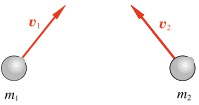
\includegraphics[width=0.41\linewidth]{Immagini/UCA 1.png}
    \quad
    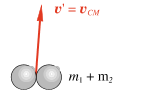
\includegraphics[width=0.3\linewidth]{Immagini/UCA 2.png}
    \caption{prima e dopo un urto completamente anelastico.}
    \label{fig: uerto completamente anelastico}
\end{figure}

Invece, l'energia cinetica prima dell'urto, applicando il secondo teorema di K\"onig, è
\begin{equation}
    K_i=\frac{1}{2}m_1v_1^2+\frac{1}{2}m_2v_2^2=K'+\frac{1}{2}(m_1+m_2)\vcm^{\ 2},
\end{equation}
mentre dopo l'urto è
\begin{equation}
    K_f=\frac{1}{2}(m_1+m_2)\vcm^{\ 2}<K_i.
\end{equation}
In effetti, dopo l'urto non è più presente moto rispetto al centro di massa, con cui i due punti coincidono, e pertanto si deduce che l'energia assorbita in questo tipo d'urto è $K'$, ossia l'energia cinetica i punti hanno rispetto al centro di massa prima dell'urto. La differenza di energia cinetica è infatti
\begin{equation}
    \Delta K=K_f-K_i=-K'.
\end{equation}
Dunque, le forze interne che si sviluppano in questo tipo di urto non sono conservative. 

\section{Urto elastico}
Un urto è elastico se nel processo si conserva anche l'energia meccanica del sistema. Questo implica necessariamente che le forze interne siano conservative. In questo tipo di urto si possono usare le relazioni
\begin{equation}
\label{eq: leggi di conservazione urto elastico}
    \vp_i=\vp_f,\quad K_i=K_f.
\end{equation}
Si consideri un urto elastico su un bersaglio nel piano. Nel sistema di riferimento del laboratorio e nel sistema di riferimento del centro di massa si hanno le situazioni mostrate in figura \ref{fig: urto elastico}.
\begin{figure}[h]
    \centering
        \begin{subfigure}{0.45\textwidth}
        \centering
        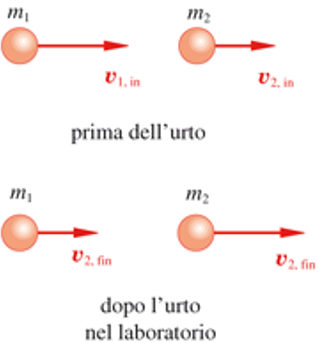
\includegraphics[width=0.8\linewidth]{Immagini/UEL.png}
        \end{subfigure}
    \quad
        \begin{subfigure}{0.45\textwidth}
        \centering
        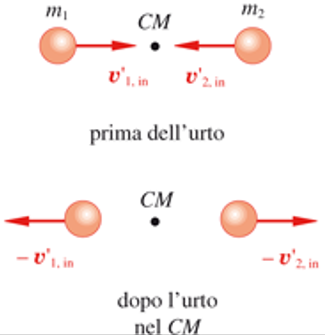
\includegraphics[width=0.8\linewidth]{Immagini/UECM.png}
        \end{subfigure}
    \caption{situazione prima e dopo l'urto nel sistema di riferimento del (i) laboratorio; (ii) centro di massa.}
    \label{fig: urto elastico}
\end{figure}

Si impongano le condizioni \eqref{eq: leggi di conservazione urto elastico} nel sistema di riferimento del laboratorio
\begin{equation}
    \begin{cases}
        \vp_{1,i}=\vp_{1,f}+\vp_{2,f} \\
        K_{1,i}=K_{1,f}+K_{2,f}
    \end{cases},
\end{equation}
che, esplicitando in termini di massa e velocità, diventano
\begin{equation}
    \begin{cases}
        m_1\vv_{1,i}=m_1\vv_{1,f}+m_2\vv_{2,f} \\[1.5ex]
        \dfrac{1}{2}m_1v_{1,i}^2=\dfrac{1}{2}m_1v_{1,f}^2+\dfrac{1}{2}m_2v_{2,f}^2
    \end{cases}.
\end{equation}
Scomponendo le velocità della prima equazione sugli assi cartesiani si ottengono
\begin{equation}
    \begin{cases}
        m_1v_{1,i}=m_1v_{1,fx}+m_2v_{2,fx} \\
        0=m_1v_{1,fy}+m_2v_{2,fy}
    \end{cases}.
\end{equation}
Quindi, si ottengono tre equazioni in quattro incognite, che sono le componenti $x$ e $y$ di $\vv_{1,f}$ e $\vv_{2,f}$. Non tutto è determinato a priori, ma c'è una dipendenza da un parametro libero che può essere identificato nell'angolo $\theta'$ di diffusione nel sistema di riferimento del centro di massa. 

Quindi, ponendosi nel sistema del centro di massa, si possono scrivere le condizioni \eqref{eq: leggi di conservazione urto elastico} come
\begin{equation}
    \begin{cases}
        m_1\vv_{1,i}'+m_2\vv_{2,i}'=m_1\vv_{1,f}'+m_2\vv_{2,f}'=0 \\[1.5ex]
        \dfrac{1}{2}m_1(\vvi_{1,i})^2+\dfrac{1}{2}m_2(\vvi_{2,i})^2=\dfrac{1}{2}m_1(\vvi_{1,f})^2+\dfrac{1}{2}m_2(\vvi_{2,f})^2
    \end{cases}.
\end{equation}
Si dimostra ora che le velocità rimangono invariate in modulo e possono ruotare solo di un angolo $\theta'$, ossia che
\begin{equation}
    v'_{1,i}=v_{1,f}',\quad v_{2,i}'=v_{2,f}'.
\end{equation}
Dalla prima equazione del sistema precedente si ottengono
\begin{equation}
    \begin{cases}
        m_1\vv_{1,i}'=-m_2\vv_{2,i}' \\
        m_1\vv_{1,f}'=-m_2\vv_{2,f}'
    \end{cases},
\end{equation}
e, se si considerano i moduli, si ottengono
\begin{equation}
    \begin{cases}
    \label{eq: sistema dimostrazione velocità urto elastico}
        v_{1,i}'=\dfrac{m_2}{m_1}v_{2,i}' \\[1.5ex]
        v_{1,f}'=\dfrac{m_2}{m_1}v_{2,f}'
    \end{cases}.
\end{equation}
Sostituendo queste nell'equazione di conservazione dell'energia cinetica si ottiene
\begin{equation}
    \begin{split}
        \dfrac{1}{2}m_1\bigg(\dfrac{m_2}{m_1}v_{2,i}'\bigg)^2+\dfrac{1}{2}m_2(\vvi_{2,i})^2&=\dfrac{1}{2}m_1\bigg(\dfrac{m_2}{m_1}v_{2,f}'\bigg)^2+\dfrac{1}{2}m_2(\vvi_{2,f})^2 \\
        \dfrac{1}{2}v_{2,i}^2\bigg(\frac{m_2^2}{m_1}+m_2\bigg)&=\dfrac{1}{2}v_{2,f}^2\bigg(\frac{m_2^2}{m_1}+m_2\bigg) \\
        (v_{2,i}')^2&=(v_{2,f}')^2 \\
        v_{2,i}'&=v_{2,f}'.
    \end{split}
\end{equation}
Sostituendo questo risultato in \eqref{eq: sistema dimostrazione velocità urto elastico} si ottiene
\begin{equation}
    v_{1,i}'=v_{1,f}'.
\end{equation}
Si è quindi dimostrato che, nel sistema del centro di massa, i modulo delle velocità sono uguali prima e dopo l'urto. Quindi, i vettori velocità possono solo ruotare di un angolo $\theta'$. Si studia ora l'urto nel sistema del centro di massa.

Prima dell'urto il centro di massa si muove solo lungo la direzione delle $x$. Usando le equazioni \eqref{eq: velocità CM} e \eqref{eq: velocità nel SdRCM}, e imponendo che il secondo corpo prima dell'urto è fermo, si ottengono
\begin{equation}
    \begin{cases}
        v_{CM}=\dfrac{m_1}{m_1+m_1}v_{1,i} \\[1.5ex]
        v_{1,i}'=\dfrac{m_2}{m_1+m_2}v_{1,i}<v_{1,i} \\[1.5ex]
        v_{2,i}'=-\dfrac{m_1}{m_1+m_2}v_{1,i}=-v_{CM}
    \end{cases}.
\end{equation}
Sostituendo la seconda equazione di questo sistema in $v_{1,i}'=v_{1,f}'$ si ottiene
\begin{equation}
    v_{1,i}'=v_{1,f}'=\dfrac{m_2}{m_1+m_2}v_{1,i}=\dfrac{m_2}{m_1+m_2}\dfrac{m_1+m_2}{m_1}v_{CM}=\frac{m_2}{m_1}v_{CM}.
\end{equation}
In modulo, usando l'equazione $v_{2,i}'=v_{2,f}'$ e l'ultima equazione del medesimo sistema si ottiene
\begin{equation}
    v_{2,i}'=v_{2,f}'=v_{CM}.
\end{equation}
Rispetto al moto del centro di massa, il primo e il secondo corpo si muovono con un angolo $\theta'$ e le loro velocità sono
\begin{equation}
    \begin{cases}
        v_{1,fx}'=\dfrac{m_2}{m_1}v_{CM}\cos{\theta'} \\[1.5ex]
        v_{1,fy}'=\dfrac{m_2}{m_1}v_{CM}\sin{\theta'}
    \end{cases},\quad
    \begin{cases}
        v_{2,fx}'=-v_{CM}\cos{\theta'} \\
        v_{2,fy}'=-v_{CM}\sin{\theta'}
    \end{cases},
\end{equation}
dove per il secondo corpo si sono usate le relazioni in \eqref{eq: sistema dimostrazione velocità urto elastico}. 

Ora passando al sistema di riferimento del laboratorio, usando l'equazione $m_1\vv_{1,i}=m_1\vv_{1,f}+m_2\vv_{2,f}$, per la situazione dopo l'urto si ha
\begin{equation}
    \begin{cases}
        v_{1,fx}=v_{CM}+\dfrac{m_2}{m_1}v_{CM}\cos{\theta'} \\
        v_{1,fy}=\dfrac{m_2}{m_1}v_{CM}\sin{\theta'}
    \end{cases},
\end{equation}
che implica, usando \eqref{eq: sistema dimostrazione velocità urto elastico}, per il secondo corpo
\begin{equation}
    \begin{cases}
        v_{2,fx}=v_{CM}(1-\cos{\theta'}) \\
        v_{2,fy}=-v_{CM}\sin{\theta'}
    \end{cases}.
\end{equation}
Il sistema del primo corpo descrive l'equazione di una circonferenza centrata in $v_x=v_{CM}$ e di raggio $r=(m_2/m_1)v_{CM}$, mentre il sistema del secondo corpo descrive l'equazione di una circonferenza centrata in $v_x=v_{CM}$ e di raggio $r=v_{CM}$. In particolare, queste sono
\begin{equation}
    \begin{cases}
        (v_{1,fx}-v_{CM})^2+(v_{1,fy}^2)=\bigg(\dfrac{m_2}{m_1}v_{CM}\bigg)^2 \\[1.5ex]
        (v_{2,fx}-v_{CM})^2+(v_{2,fy})^2=(v_{CM})^2
    \end{cases}.
\end{equation}
Si presentano tre casi:
\begin{enumerate}
    \item Se il bersaglio è pesante, ossia $m_2>m_1$, allora il proiettile può tornare indietro (Rutherford).
    \item Se il bersaglio ha la stessa massa del proiettile, ossia $m_1=m_2$, allora il proiettile può fermarsi (Fermi).
    \item Se il bersaglio è leggero, ossia $m_1>m_2$, allora il proiettile non torna mai indietro, ma solo in avanti.
\end{enumerate}

\section{Urto anelastico}
Il caso di urto più comune si verifica quando i due punti materiali, dopo aver colliso, tornano ad essere separati. Se non agiscono forze esterne di tipo impulsivo, la quantità di moto si conserva, ma non l'energia cinetica. Una certa frazione $K'$, l'energia cinetica prima dell'urto rispetto al centro di massa, viene assorbita. 


Si consideri un urto elastico nel sistema di riferimento del centro di massa. Il punto con quantità di moto $\vpi_{1,i}$ nell'istante precedente all'urto vede, per effetto dell'impulso nella fase di deformazione, ridursi la quantità di moto progressivamente a zero fino ad arrestarsi. Nella fase successiva, sempre durante l'urto, il punto riacquista quantità di moto fino al valore $\vpi_{1,f}$, opposto in verso e minore di $\vpi_{1,i}$. Si definisce il coefficiente di restituzione $\epsilon$ il rapporto
\begin{equation}
    \epsilon=-\frac{\vpi_{1,f}}{\vpi_{1,i}}=-\frac{\vvi_{1,f}}{\vvi_{1,i}}=-\frac{\vpi_{2,f}}{\vpi_{2,i}}=-\frac{\vvi_{2,f}}{\vvi_{2,i}}.
\end{equation}
Infatti, dato che $\vp=0$, in modulo $p_{1,i}'=p_{2,i}'$ e $p_{1,f}'=p_{2,f}'$, per cui il coefficiente di restituzione è lo stesso anche per la seconda particella. L'energia cinetica del sistema delle due particelle dopo l'urto è
\begin{equation}
    K_f'=\frac{1}{2}m_1(v'_{1,f})^2+\frac{1}{2}m_2(v'_{2,f})^2=\epsilon^2\bigg[\frac{1}{2}m_1(v'_{1,i})^2+\frac{1}{2}m_2(v'_{2,i})^2\bigg]=\epsilon^2K_i'.
\end{equation}
La variazione relativa di energia cinetica rispetto al centro di massa nell'urto è
\begin{equation}
    \delta=\frac{K_f'-K_i'}{K_i'}=\epsilon^2-1.
\end{equation}
Nell'urto elastico $\epsilon=1$ e $\delta=0$, nell'urto completamente anelastico $\epsilon=0$ e $\delta=-1$. Nella situazione di urto anelastico, il coefficiente di restituzione risulta $\epsilon\in(0,1)$, mentre $K_f'<K_i'$. 

La soluzione per le velocità finali nel sistema di riferimento inerziale, sempre nel caso di urto centrale come per l'urto elastico, risulta
\begin{align}
    v_{1,f}&=\frac{(m_1-\epsilon m_2)v_{1,i}+m_2(1+\epsilon)v_{2,i}}{m_1+m_2}, \\
    v_{2,f}&=\frac{m_1(1+\epsilon)v_{1,i}+(m_2-\epsilon m_1)v_{2,i}}{m_1+m_2}.
\end{align}
Con $\epsilon=1$ e $\epsilon=0$ si ritrovano infatti le relazioni per il caso elastico e completamente anelastico. 

\section{Urto con corpi rigidi}
Un urto può anche avvenire tra un punto materiale e un corpo rigido oppure tra due (o più) corpi rigidi. Riassumendo, in un urto si può assumere la costanza dell'energia cinetica del sistema solo se è noto a priori che l'urto è elastico. Se agiscono solo forze interne, o quelle esterne non sono di tipo impulsivo, si conserva la quantità di moto totale. Se invece esiste un vincolo che tiene fermo un punto del corpo rigido, e quindi sviluppa una forza esterna di tipo impulsivo durante l'urto, non si verifica la conservazione della quantità di moto. Infine, qualora rispetto a un certo polo, fisso in un sistema di riferimento inerziale o coincidente con il centro di massa, il momento delle forze esterne, comprese quelle vincolari è nullo, si  conserva il momento angolare rispetto a tale polo. Se agiscono solo forze interne $\vL$ si conserva sempre, indipendentemente dalla scelta del polo.

Quando il corpo urtato è vincolato, il sistema di vincoli può esplicare durante l'urto un sistema di forze che ha una risultante $\vR$ e un momento risultante $\vM$. L'effetto complessivo, nel brevissimo tempo di durata dell'urto, è dato dall'impulso della forza $J=\int\vR\,dt$ e dall'impulso angolare $\Delta L=\int\vM\,dt$, eguali rispettivamente alla variazione della quantità di moto e alla variazione del momento angolare del sistema.

Essendo la quantità di moto e il momento angolare grandezze vettoriali, è possibile trovare situazioni in cui la loro conservazione è parziale; per esempio, $p_x$ e $p_y$ si conservano, $p_z$ cambia: questo vuol dire che l'impulso ha componenti $J_x$ e $J_y$ nulle, mentre $J_z$ è diversa da zero. Analogamente per $\vL$ e l'impulso angolare.
\begin{figure}[h]
    \centering
    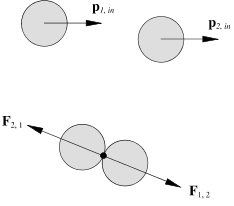
\includegraphics[width=0.3\linewidth]{Immagini/UCR 1.png}
    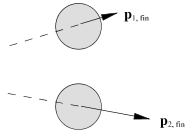
\includegraphics[width=0.3\linewidth]{Immagini/UCR 2.png}
    \caption{urto tra due corpi rigidi non ruotanti (i) prima dell'urto; (ii) durante l'urto; (iii) dopo l'urto.}
    \label{fig: urto corpi rigidi}
\end{figure}

Quando due corpi estesi si urtano, ma non restano attaccati, le quantità di moto dopo l'urto formano normalmente un certo angolo con la direzione che avevano prima dell'urto. Infatti la forza interna impulsiva $\vF_{2,1}$ agente sul primo corpo non è parallela a $\vp_{1,i}$ e quindi $\vp_{1,f}$ risulta deviata rispetto alla direzione iniziale del moto; lo stesso succede per il secondo corpo. La situazione è mostrata qualitativamente in figura \ref{fig: urto corpi rigidi} riferita a due dischetti che non ruotano prima dell'urto. Essi non ruotano nemmeno dopo se non c'è attrito al contatto, cioè se le forze interne non hanno componente tangente. Altrimenti il momento dell'attrito mette in rotazione i dischetti. Solo se i centri dei due dischetti si muovono lungo la stessa retta non si ha deviazione e si parla di urto centrale; l'urto della \ref{fig: urto corpi rigidi} non è centrale.